\documentclass[11pt]{article}
\usepackage[margin=1.5in]{geometry}
\usepackage{graphicx}
\usepackage{float}
\usepackage{parskip}
\usepackage{amsmath}
\usepackage{pgfplots}
\pgfplotsset{width=10cm, compat=1.9}

\begin{document}

\textbf{\Huge Analytical Applications of \\ Derivatives}

Athan Zhang \& Jeffrey Chen

\section{Local Linear Approximation}
Derivatives can also be used to approximate nonlinear functions using the tangent line. Simply put, the tangent line to the curve $f(x)$ at point $x=x_0$ is called the \textbf{local linear approximation} of $f(x)$ at $x=x_0$: 

\[f(x) \approx f(x_0)+f'(x_0)(x-x_0)\]

This approximation can be used to estimate the value of $f(x)$ at values close to $x_0$. Logically, the farther away you get from $x_0$, the less accurate your estimate will be. 

For example, the local linear approximation of $y=x^2+2$ at $x=1$ can be used to approximate the value of the curve at $x=1.5$:

\begin{center}
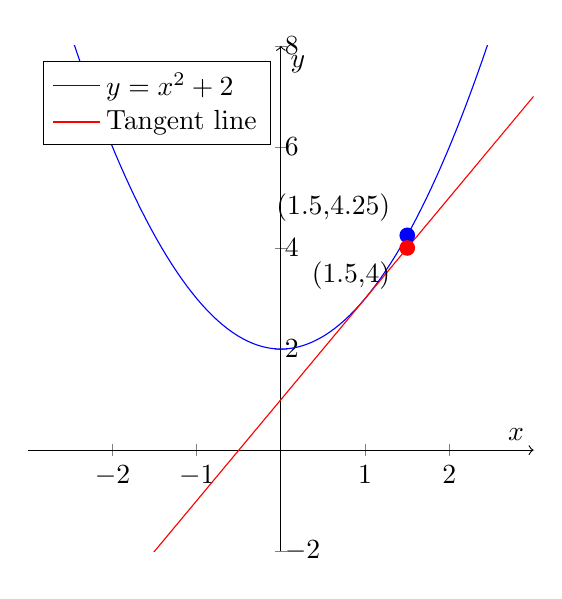
\begin{tikzpicture}
  \begin{axis}[
    xlabel={$x$},
    ylabel={$y$},
    xmin=-3, xmax=3,
    ymin=-2, ymax=8,
    width=8cm, height=8cm,
    axis lines=middle,
    axis line style={->},
    xtick={-2,-1,0,1,2},
    ytick={-2,0,2,4,6,8},
    yticklabel style={anchor=west},
    legend pos=north west,
    legend cell align={left},
  ]

  \addplot[blue, domain=-3:3, samples=100] {x^2 + 2};

  \addplot[red, domain=-3:3, samples=2] {2*x + 1};
  \node[blue, label={150:{(1.5,4.25)}},circle,fill,inner sep=2pt] at (axis cs:1.5,4.25) {};
  \node[red, label={210:{(1.5,4)}},circle,fill,inner sep=2pt] at (axis cs:1.5,4) {};
  \legend{$y = x^2 + 2$, Tangent line}

  \end{axis}
\end{tikzpicture}
\end{center}

However, the approximation becomes less accurate for $x=2$:

\begin{center}
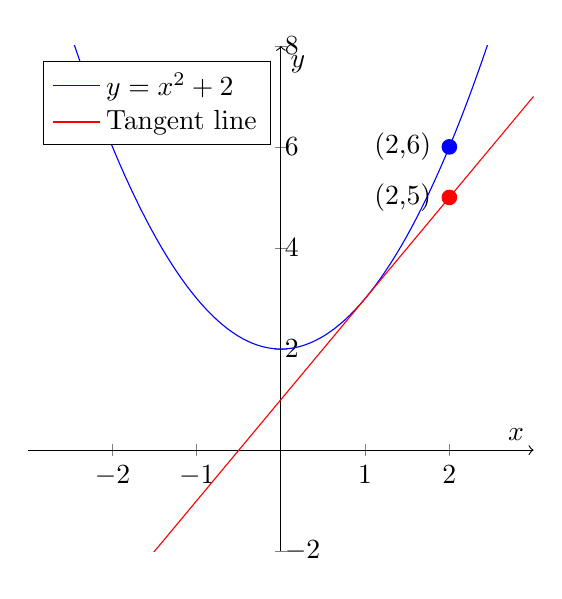
\begin{tikzpicture}
  \begin{axis}[
    xlabel={$x$},
    ylabel={$y$},
    xmin=-3, xmax=3,
    ymin=-2, ymax=8,
    width=8cm, height=8cm,
    axis lines=middle,
    axis line style={->},
    xtick={-2,-1,0,1,2},
    ytick={-2,0,2,4,6,8},
    yticklabel style={anchor=west},
    legend pos=north west,
    legend cell align={left},
  ]

  \addplot[blue, domain=-3:3, samples=100] {x^2 + 2};

  \addplot[red, domain=-3:3, samples=2] {2*x + 1};
  \node[blue, label={180:{(2,6)}},circle,fill,inner sep=2pt] at (axis cs:2,6) {};
  \node[red, label={180:{(2,5)}},circle,fill,inner sep=2pt] at (axis cs:2,5) {};
  \legend{$y = x^2 + 2$, Tangent line}

  \end{axis}
\end{tikzpicture}
\end{center}

% add example

\section{Analysis of Functions}
Derivatives can be used to extensively analyze functions. We will cover some examples of the possible analysis in the sections below.

\subsection{Concavity}
Obviously, a function's derivative being positive on an interval implies the function is increasing on that interval, and a negative derivative implies decreasing. However, we can also analyze the \textbf{concavity} of a function based on derivatives. 

A function is said to be \textbf{concave up} on an interval if its second derivative is positive on said interval. Likewise, it is said to be \textbf{concave down} on an interval if its second derivative is negative on said interval.

A point where a function changes concavity is called an \textbf{inflection point}. Note that the second derivative equalling zero at a point is necessary but \textbf{not sufficient} for that point to be an inflection point; the second derivative must change signs as well. 

\subsection{Relative Extrema}
A function $f(x)$ is said to have a \textbf{relative extremum} at point $x_0$ if there exists an interval containing $x_0$ on which $f(x_0)$ is either the smallest or largest value on the interval.

Derivatives can be used to find relative extrema of smooth curves, due to the fact that these extrema occur at peaks and valleys of the curve where the tangent line is horizontal, also known as \textbf{critical points}. By setting the derivative of a function equal to zero and solving for all solutions on an interval, we can obtain the critical points on that interval. 

Next, in order to determine which critical points are relative extrema, we follow this set of rules known as the \textbf{first derivative test}, assuming $c$ is a critical point of the function: 

\begin{enumerate}
  \item If \(f'(x) > 0\) to the left of \(c\) and \(f'(x) < 0\) to the right of \(c\), then \(f(c)\) has a relative maximum at \(c\).
  \item If \(f'(x) < 0\) to the left of \(c\) and \(f'(x) > 0\) to the right of \(c\), then \(f(c)\) has a relative minimum at \(c\).
  \item If the signs of \(f'(x)\) do not change, the first derivative test is inconclusive.
\end{enumerate}

There is a second method for determining relative extrema using derivatives, known as the \textbf{second derivative test}, which states the following, assuming $c$ is a critical point of the function: 

\begin{enumerate}
  \item If \(f''(c) > 0\), then \(f(c)\) has a relative minimum at \(c\).
  \item If \(f''(c) < 0\), then \(f(c)\) has a relative maximum at \(c\).
  \item If \(f''(c) = 0\), the second derivative test is inconclusive.
\end{enumerate}

Notice that for smooth curves, while relative extrema are guaranteed to occur at only critical points, not every critical point is guaranteed to be a relative extremum.

\subsection{Absolute Extrema}
A function $f(x)$ is said to have an \textbf{absolute extremum} at point $x_0$ on an interval if $f(x_0)$ is either the smallest or largest value on the interval. Notice that there can be multiple relative extrema on an interval, but at most \textbf{one} absolute maximum value and \textbf{one} absolute minimum value.

The process for determining absolute extrema, like before, involves first finding all critical points of a function on a given interval. Next, the value of the function at every critical point must be determined, and the point where the largest value occurs is the absolute maximum, and the point where the smallest value occurs is the absolute minimum.

\subsection{Contextual Applications of Analysis}
There are many contextual applications of the topics and techniques discussed above. Finding relative and absolute extrema is an important ability in countless scenarios. For example:

Suppose a car's position can be modeled as $\frac{1}{4}t^4-2t^3+\frac{9}{2}t^2+t$, where $t$ represents the number of seconds passed from now. What is the minimum velocity the car will reach, and when will it occur?

To solve this problem and others like it, the relative and/or absolute extrema of the function must be analyzed using derivatives. How would you solve this problem?

\section{L'Hopital's Rule}
Another analytical application of derivatives lies in finding limits that would otherwise be impossible to find. The rule is stated as follows: 

If $\lim_{x \to a} f(x) = \lim_{x \to a} g(x) = 0$ or $\lim_{x \to a} f(x) = \lim_{x \to a} g(x) = \pm \infty$, and $\lim_{x \to a} \frac{f'(x)}{g'(x)}$ exists (or equals $\pm \infty$), then

\[\lim_{x \to a} \frac{f(x)}{g(x)} = \lim_{x \to a} \frac{f'(x)}{g'(x)}\]

This rule essentially allows us to replace the original limit with a new limit involving the derivatives of the functions. It is important to note that L'Hopital's Rule applies only when the given limit is in an \textbf{indeterminate form} such as $\frac{0}{0}$ or $\frac{\infty}{\infty}$.

\section{Newton's Method}
Students may already know some methods for approximating the zeroes of a function, such as Intermediate Value Theorem. However, Newton's Method, an iterative method which utilizes derivatives, is much more efficient than previously learned methods, and is commonly used by modern computers to approximate zeroes of functions.

Suppose we want to approximate a zero $a$ of the function $f(x)$. First, we must pick a general approximation, $x_1$. Then, we can infinitely iterate with the following formula to produce more and more accurate approximations of $a$:

\[ x_{n+1} = x_n - \frac{f(x_n)}{f'(x_n)}\]

If infinite iterations are calculated, $x_n$ should theoretically converge to $a$ in most cases. However, the convergence occurs quickly, so under normal circumstances, only a few iterations are necessary to produce an acceptably accurate approximation.

Notice that Newton's method is not guaranteed to produce results in every case; sometimes it may not converge, or sometimes it may completely skip the zero of interest and converge to a different, nearby zero. However, it is still a powerful tool for approximating zeroes in most cases.

\section{Rolle's Theorem and Mean Value Theorem}
Rolle's Theorem is a special case of a more general theorem, the Mean Value Theorem. Neither of these theorems have extensive uses in application problems, but they are used in proofs of many of the results we have already covered in the course, so they are nevertheless regarded as some of the most important principles of calculus.

\subsection{Rolle's Theorem}
Let \(f(x)\) be a function that satisfies the following conditions:

\begin{enumerate}
  \item \(f(x)\) is continuous on the closed interval \([a, b]\).
  \item \(f(x)\) is differentiable on the open interval \((a, b)\).
  \item \(f(a) = f(b)\).
\end{enumerate}

Then, there exists at least one point \(c\) in the open interval \((a, b)\) such that \(f'(c) = 0\).

In other words, Rolle's Theorem states that if a function is continuous on a closed interval and differentiable on the corresponding open interval, and the function has the same value at the endpoints of the interval, then there exists at least one point within the interval where the derivative of the function is zero.

\subsection{Mean Value Theorem}
Let \(f(x)\) be a function that satisfies the following conditions:

\begin{enumerate}
  \item \(f(x)\) is continuous on the closed interval \([a, b]\).
  \item \(f(x)\) is differentiable on the open interval \((a, b)\).
\end{enumerate}

Then, there exists at least one point \(c\) in the open interval \((a, b)\) such that the derivative of \(f(x)\) at \(c\), denoted as \(f'(c)\), is equal to the average rate of change of \(f(x)\) over the interval \([a, b]\), which is given by:

\[
f'(c) = \frac{{f(b) - f(a)}}{{b - a}}
\]

In other words, the Mean Value Theorem states that for any continuous and differentiable function on a closed interval, there exists a point within the interval where the instantaneous rate of change (the derivative) is equal to the average rate of change of the function over the interval.
\end{document}